\documentclass[titlepage]{article}
\usepackage[utf8]{inputenc}
\usepackage[T1]{fontenc}
\usepackage{graphicx}
\usepackage{caption} 
\usepackage{listings}
\usepackage{xcolor}

\title{Rapport MT10 - TP2 : Autour du RSA}
\author{Martin Schneider, Océane Bordeau}
\date{10 mai 2022}

\setlength{\parindent}{0pt}
\definecolor{codegreen}{rgb}{0,0.6,0}
\definecolor{codegray}{rgb}{0.5,0.5,0.5}
\definecolor{codepurple}{rgb}{0.58,0,0.82}
\definecolor{codeblue}{rgb}{0,0,255}
\definecolor{backcolour}{rgb}{0.95,0.95,0.92}

\lstdefinestyle{mystyle}{ 
    commentstyle=\color{magenta},
    keywordstyle=\color{codeblue},
    numberstyle=\tiny\color{codegray},
    stringstyle=\color{codepurple},
    basicstyle=\ttfamily\footnotesize,
    breakatwhitespace=false,         
    breaklines=true,                 
    captionpos=b,                    
    keepspaces=true,                                  
    showspaces=false,                
    showstringspaces=false,
    showtabs=false,                  
    tabsize=2
}

\lstset{style=mystyle}

\begin{document}
    \maketitle
    \tableofcontents
    \pagebreak

    \section{Préliminaire : \texttt{SageMath} et les nombres entiers}

    \section{Nombres premiers}
    \subsection{Sur la répartition des nombres premiers}
    \bigbreak
    L’objectif est d’observer le comportement de suite $u_n = \pi(n)\frac{\ln n}{n}$, pour des n les plus grands possibles.
    \bigbreak
    1. Jusqu'à $10^{13}$, la commande \texttt{prime\_pi} met moins d'une dizaine de seconde à s'éxécuter, pour $10^{14}$, l'éxécution prend envirion 55 secondes. La limite de la minute est atteinte pour $10^{15}$.
    \bigbreak
    2. $\pi (n)$ désigne les nombres premiers $\leq n$.\newline
    Traçons sur un même graphique $n \mapsto \pi (n)$ et $n \mapsto \frac{n}{\ln n}$ :  
    \begin{center}
        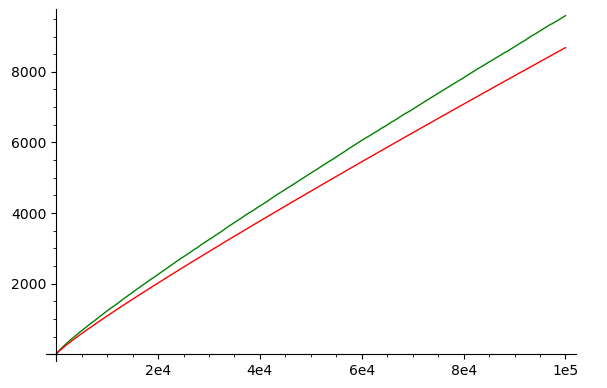
\includegraphics[scale=0.5]{Ressources/2022-04-27-10:20:27-screenshot.png}
        \captionof{figure}{}
        \end{center}
    \bigbreak
    3. Traçons $u_n$ en fonction de $n$ : 
    \begin{center}
        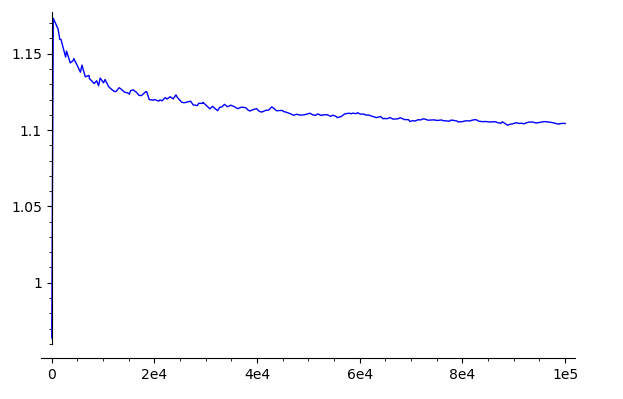
\includegraphics[scale=0.5]{Ressources/2022-04-27-10:20:31-screenshot.png}
        \captionof{figure}{}
    \end{center}
    \bigbreak



    \subsection{Nombres de Fermat}

    \subsection{Nombres de Mersenne}

    \subsection{Un test de primalité pour les nombres de Mersenne}

    \section{Algorithmes d'exponentiation}
    \subsection{Naïf itératif et naïf récursif}

    \subsection{Dichotomique itératif et dichotomique récursif}

    \subsection{Algorithme d'exponentiation modulaire}

\end{document}
